\documentclass{standalone}
\usepackage{hsbcommon}
\begin{document}
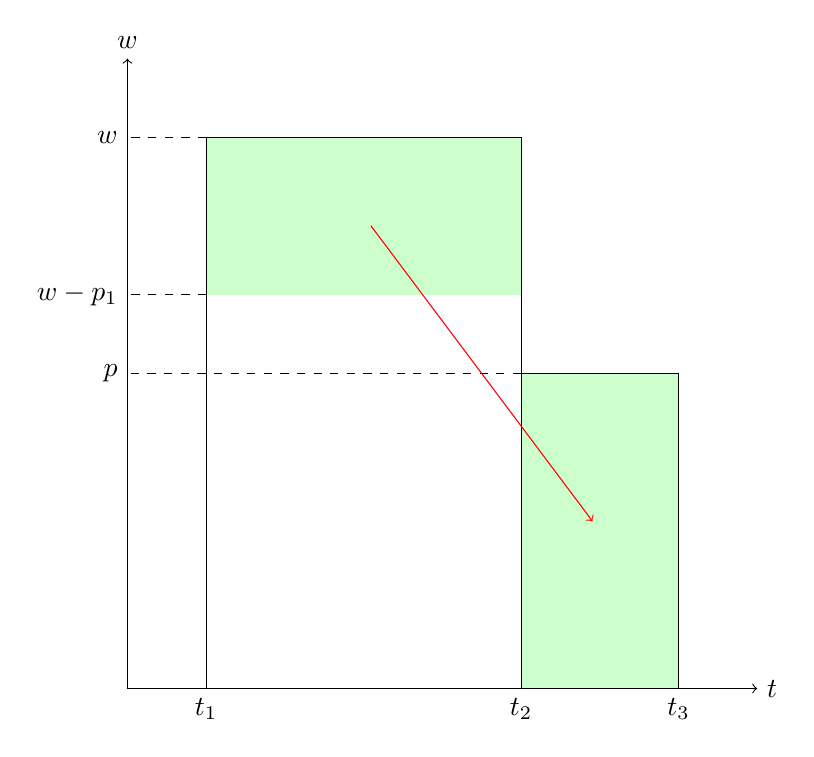
\begin{tikzpicture}

    \draw[->] (0,0) -- (8,0) node[right] {$t$};
    \draw[->] (0,0) -- (0,8) node[above] {$w$};

    
    \fill[green!20] (1,5) rectangle node(A){} (5,7);  % 4*2
    \draw (1,0) rectangle (5,7);
    
    \draw[fill=green!20] (5,0) rectangle node(B){} (7,4); % 2*4

    \draw[dashed] (1,7) -- (0,7) node[left] {$w$};
    \draw[dashed] (1,5) -- (0,5) node[left] {$w-p_1$};
    
    \draw[dashed] (5,4) -- (0,4) node[left] {$p$};

    \node[below] at (1,0) {$t_1$};
    \node[below] at (5,0) {$t_2$};
    \node[below] at (7,0) {$t_3$};

    \draw[red,->] (A) -- (B);
    

\end{tikzpicture}

\end{document}